\documentclass[12pt,a4paper]{article}

\usepackage[margin=1in]{geometry}
\usepackage{graphicx}
\usepackage{float}
\usepackage{booktabs}
\usepackage{array}
\usepackage{longtable}
\usepackage{amsmath}
\usepackage{tikz}
\usepackage{hyperref}
\usepackage{caption}
\usepackage{setspace}
\usepackage{enumitem}
\usepackage{cite}
\usetikzlibrary{arrows.meta,positioning,shapes.geometric,fit}

\hypersetup{
  colorlinks=true,
  linkcolor=black,
  citecolor=black,
  urlcolor=blue
}

\setstretch{1.15}

\begin{document}

% ------------------------
% Cover Page
% ------------------------
\begin{titlepage}
    \centering

    \vspace*{0.8cm}
    
\includegraphics[width=0.20\textwidth]{figures/MIST_Logo.png}\\[0.8cm]

    {\Large \textbf{Military Institute of Science and Technology}}\\[0.2cm]
    {\large Department of Computer Science and Engineering}\\[1.0cm]

    

    \begin{tabular}{>{\bfseries}p{4cm} p{10cm}}
        Project Title: & Competition Certificate Verification using CNN\\
        Course ID: & CSE-404 \\
        Group No.: & B3 \\
        Submission Date: & 29/03/2026 \\
    \end{tabular}

    \vspace{0.8cm}
    \textbf{Member Names and IDs}

    \vspace{0.4cm}
    \begin{tabular}{|c|l|c|}
        \hline
        No. & Name & Student ID \\
        \hline
        1 & Shaikh Sabah Taj Shefa & 202114181 \\
        2 & Nahidur Zaman & 202214075 \\
        3 & Sakif Shahrear & 202214093 \\
        4 & Syed Mafijul Islam & 202214105 \\
        \hline
    \end{tabular}

    \vfill
    {\large Final Project Report}
\end{titlepage}

% ------------------------
% Abstract
% ------------------------
\section*{Abstract}
Certificate forgery has become increasingly easy with modern image editing tools, while manual verification remains slow and error-prone. This project presents an automated binary image-classification system for distinguishing real and fake competition certificates using a Convolutional Neural Network (CNN). A custom dataset of 200 RGB images was used, containing 126 real and 74 fake certificates. The dataset was split using stratified sampling into training and validation sets, resized to $128 \times 128$, normalized to $[0,1]$, and augmented with random rotation and horizontal flipping. The implemented CNN consists of three convolutional blocks followed by dense layers and was trained with Adam optimizer and binary cross-entropy loss. In the recorded run, the model achieved approximately $67.4\%$ validation accuracy. Confusion-matrix analysis shows that genuine certificates were detected strongly, but fake certificates were frequently misclassified as real, indicating a class-bias issue. This behavior highlights the need for stronger forgery-focused feature learning and better class balancing. Overall, the project demonstrates a practical end-to-end pipeline for automated certificate screening and establishes a baseline that can be improved through transfer learning, improved sampling strategy, and expanded forgery diversity.

\newpage
\tableofcontents
\newpage

% ------------------------
% 1. Introduction
% ------------------------
\section{Introduction}
\subsection{Problem Statement}
In the current competitive environment, certificates from hackathons, coding competitions, and workshops are vital proof of a student's or professional's extra-curricular skills. However, the rise of user-friendly digital editing tools like Canva and Photoshop has made it extremely easy to forge these competition certificates. Fraudsters often take an original template from a well-known event and simply change the name, rank, or date to create a fake version. These pixel-level manipulations, such as mismatched font textures or slightly altered logos, are almost impossible for the human eye to detect during a quick manual review. Traditional verification via QR codes or manual emails to organizers is often slow and sometimes impossible if the organizers do not maintain a permanent database. Therefore, there is an urgent need for an automated, AI-based visual verification system that can instantly analyze a competition certificate image and classify it as real or fake based on its structural and textural integrity.

\subsection{Significance of the Project}
The significance of this project lies in its ability to protect the credibility of genuine achievements in the competitive landscape:
\begin{itemize}[leftmargin=*]
    \item Integrity of competitions: It ensures that the hard work of actual winners is protected by identifying and filtering out fraudulent claims of participation or winning.
    \item Instant verification: Unlike manual verification which can take days, this CNN-based model provides a result in seconds, making it ideal for high-volume screening during job recruitments or university admissions.
    \item Texture-based detection: By using deep learning, the system identifies forgery signatures such as subtle blurring around edited text, inconsistent noise patterns, and font alignment errors that occur during digital tampering.
    \item Low-cost and scalable: It provides a lightweight alternative to expensive blockchain-based systems, allowing even small-scale event organizers to use AI for securing their certificates.
    \item Accessible technology: The use of MobileNetV2-inspired lightweight design choices makes the model efficient enough for future deployment on mobile devices, allowing certificate checks on the go.
\end{itemize}

% ------------------------
% 2. Literature Review
% ------------------------
\section{Literature Review}
Common digital certificate checking methods use central portals, digital signatures, and blockchain \cite{fastver2025,semantic2023}. These methods are secure, but they can be hard to set up and use. The table below compares the two papers used in this project.

\begin{table}[H]
\centering
\renewcommand{\arraystretch}{1.25}
\resizebox{\textwidth}{!}{%
\begin{tabular}{|p{2.8cm}|p{4.6cm}|p{4.2cm}|p{4.0cm}|}
\hline
\textbf{Paper} & \textbf{Focus} & \textbf{Problem} & \textbf{Missing Need} \\
\hline
Fake Me If You Can (FastVer, SFastVer) \cite{fastver2025} & Blockchain-based systems, PKI/digital signature approaches, third-party verification, and local certificate portals for authenticity checking. & High cost and complexity of blockchain, slow manual verification, no global interoperability, inefficient revocation system, and trust management problems. & No instant verification system, no low-cost alternative to blockchain, lack of a global scalable framework, and no efficient certificate revocation method. \\
\hline
Semantic Scholar paper \cite{semantic2023} & Traditional manual verification, blockchain-based verification, digital signature systems, and centralized trusted-authority models. & Slow and inefficient verification, high implementation cost, scalability issues, cross-border verification challenges, and privacy/data-sharing concerns. & Need for fast and automated verification, lack of a lightweight and scalable solution, no proper global verification framework, and need for a secure but low-cost system. \\
\hline
\end{tabular}%
}
% Literature table intentionally has no caption or numbering.
\end{table}

\subsection{Research Gap}
Both papers show that a faster and more practical method is needed. This project fills that need by using image-based deep learning to spot fake competition certificates from visual clues, without using an external database.

% ------------------------
% 3. Dataset Description
% ------------------------
\section{Dataset Description}
\subsection{Source and Composition}
Metadata was prepared by scanning two folders (\texttt{real} and \texttt{fake}) and assigning labels based on directory source. Total samples: 200 images.

\subsection{Class Distribution}
\begin{itemize}[leftmargin=*]
    \item Real: 126
    \item Fake: 74
\end{itemize}
A stratified 80:20 split was applied:
\begin{itemize}[leftmargin=*]
    \item Training: 160 (Real: 101, Fake: 59)
    \item Validation: 40 (Real: 25, Fake: 15)
\end{itemize}

\begin{figure}[H]
    \centering
    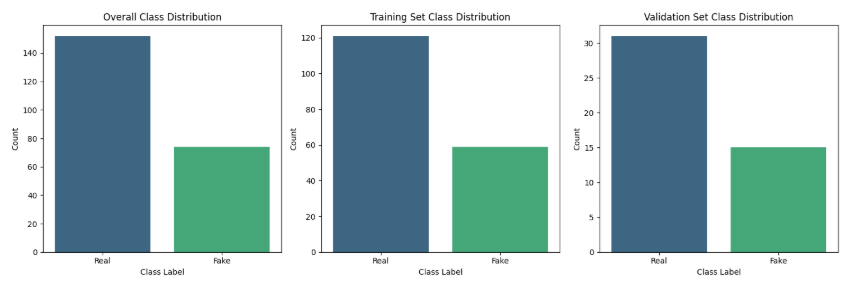
\includegraphics[width=0.95\textwidth]{figures/dataset_description_1.png}
    \caption{Overall, training, and validation class distributions.}
\end{figure}

\subsection{Preprocessing and Augmentation}
\begin{itemize}[leftmargin=*]
    \item Resize to $128 \times 128$ RGB.
    \item Pixel rescaling using $1/255$ normalization.
    \item Training augmentation: rotation range $20^{\circ}$ and horizontal flip.
    \item Validation generator uses only rescaling (no augmentation).
\end{itemize}

% ------------------------
% 4. Methodology
% ------------------------
\section{Methodology}
\subsection{Abstract Diagram}
\begin{figure}[H]
\centering
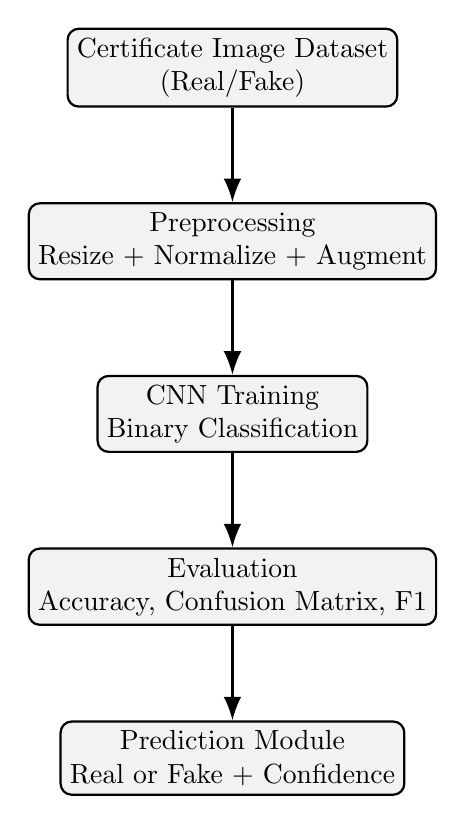
\begin{tikzpicture}[
    node distance=1.2cm and 0.8cm,
    block/.style={rectangle, rounded corners, draw=black, thick, align=center, minimum height=0.9cm, minimum width=3.0cm, fill=gray!10},
    arrow/.style={-{Latex[length=3mm]}, thick}
]
\node[block] (data) {Certificate Image Dataset\\(Real/Fake)};
\node[block, below=of data] (prep) {Preprocessing\\Resize + Normalize + Augment};
\node[block, below=of prep] (train) {CNN Training\\Binary Classification};
\node[block, below=of train] (eval) {Evaluation\\Accuracy, Confusion Matrix, F1};
\node[block, below=of eval] (infer) {Prediction Module\\Real or Fake + Confidence};

\draw[arrow] (data) -- (prep);
\draw[arrow] (prep) -- (train);
\draw[arrow] (train) -- (eval);
\draw[arrow] (eval) -- (infer);
\end{tikzpicture}
\caption{End-to-end methodological flow from data to certificate prediction.}
\end{figure}

\subsection{Model Architecture and Layer Details}
The model uses a custom Sequential CNN:
\begin{itemize}[leftmargin=*]
    \item Input: $128 \times 128 \times 3$
    \item Conv2D (32, $3 \times 3$, ReLU) + MaxPool($2 \times 2$)
    \item Conv2D (64, $3 \times 3$, ReLU) + MaxPool($2 \times 2$)
    \item Conv2D (128, $3 \times 3$, ReLU) + MaxPool($2 \times 2$)
    \item Flatten
    \item Dense(128, ReLU)
    \item Dense(1, Sigmoid)
\end{itemize}

\begin{figure}[H]
\centering
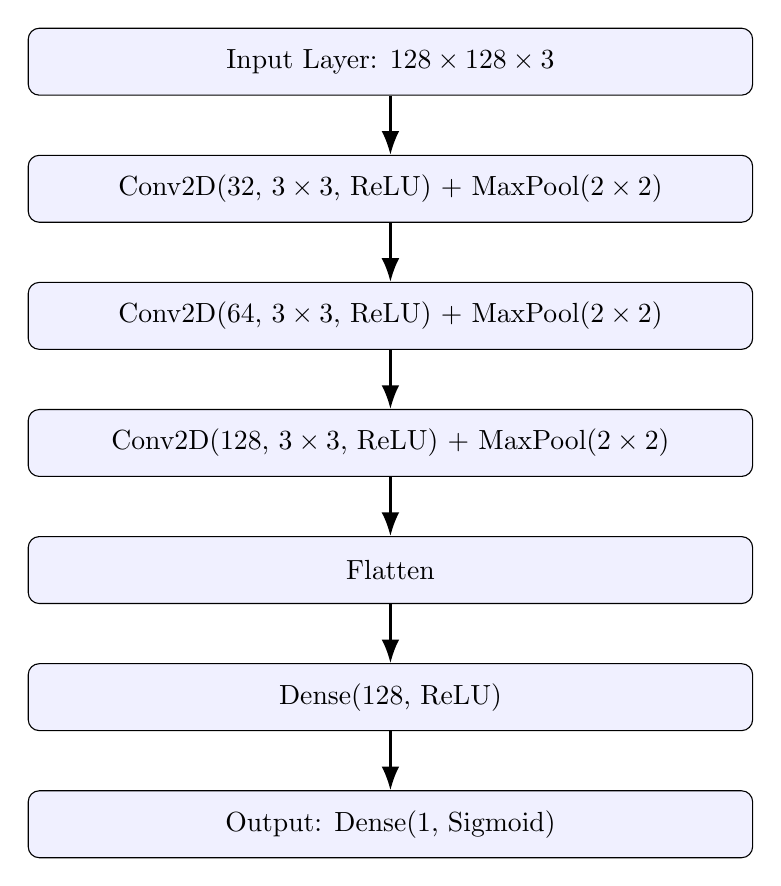
\begin{tikzpicture}[
    node distance=0.75cm,
    layer/.style={rectangle, draw=black, rounded corners, minimum height=0.85cm, minimum width=9.2cm, align=center, fill=blue!6},
    arrow/.style={-{Latex[length=3mm]}, thick}
]
\node[layer] (l1) {Input Layer: $128 \times 128 \times 3$};
\node[layer, below=of l1] (l2) {Conv2D(32, $3\times3$, ReLU) + MaxPool($2\times2$)};
\node[layer, below=of l2] (l3) {Conv2D(64, $3\times3$, ReLU) + MaxPool($2\times2$)};
\node[layer, below=of l3] (l4) {Conv2D(128, $3\times3$, ReLU) + MaxPool($2\times2$)};
\node[layer, below=of l4] (l5) {Flatten};
\node[layer, below=of l5] (l6) {Dense(128, ReLU)};
\node[layer, below=of l6] (l7) {Output: Dense(1, Sigmoid)};

\draw[arrow] (l1) -- (l2);
\draw[arrow] (l2) -- (l3);
\draw[arrow] (l3) -- (l4);
\draw[arrow] (l4) -- (l5);
\draw[arrow] (l5) -- (l6);
\draw[arrow] (l6) -- (l7);
\end{tikzpicture}
\caption{CNN architecture used in this project.}
\end{figure}

\subsection{Technical Rationale}
Small-kernel convolutions are used to capture local texture and edge anomalies introduced by forgery edits. Pooling layers reduce spatial dimension and overfitting risk. Sigmoid output with binary cross-entropy aligns with two-class classification.

% ------------------------
% 5. Experimental Setup
% ------------------------
\section{Experimental Setup}
\subsection{Hardware}
\begin{itemize}[leftmargin=*]
    \item Platform: Google Colab
    \item GPU: NVIDIA T4 (16 GB)
    \item RAM: 12.7 GB
    \item CPU: Intel Xeon 2.20 GHz
\end{itemize}

\subsection{Software}
\begin{itemize}[leftmargin=*]
    \item Python
    \item TensorFlow/Keras
    \item Pandas, NumPy
    \item Scikit-learn
    \item Matplotlib, Seaborn, Plotly
\end{itemize}

\subsection{Hyperparameters}
\begin{table}[H]
\centering
\begin{tabular}{ll}
\toprule
Parameter & Value \\
\midrule
Input size & $128 \times 128 \times 3$ \\
Batch size & 32 \\
Epochs & 10 \\
Optimizer & Adam \\
Learning rate & 0.001 \\
Loss function & Binary cross-entropy \\
Train/Validation split & 80\% / 20\% (stratified) \\
\bottomrule
\end{tabular}
\caption{Training configuration}
\end{table}

% ------------------------
% 6. Result Analysis
% ------------------------
\section{Result Analysis}
\subsection{Training Curves}
\begin{figure}[H]
    \centering
    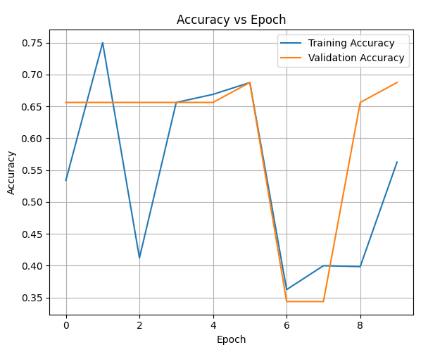
\includegraphics[width=0.75\textwidth]{figures/Accuracy_VS_epoch_1.png}
    \caption{Training and validation accuracy over 10 epochs.}
\end{figure}

\begin{figure}[H]
    \centering
    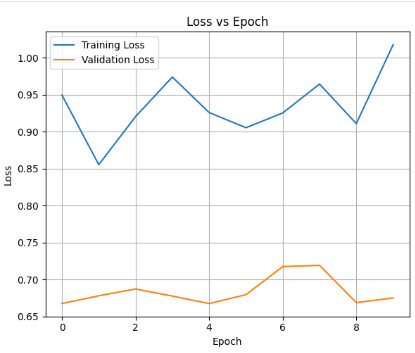
\includegraphics[width=0.75\textwidth]{figures/Loss_VS_Epoch_1.png}
    \caption{Training and validation loss over 10 epochs.}
\end{figure}

Validation accuracy remains around $0.656$ during training history, while training accuracy fluctuates. This suggests unstable generalization and possible underfitting of fake-certificate patterns.

\subsection{Classification Metrics}
From the saved confusion matrix figure (validation support: 46 samples), the matrix is:
\[
\begin{bmatrix}
0 & 15 \\
0 & 31
\end{bmatrix}
\]
(rows: true labels [Fake, Real], columns: predicted labels [Fake, Real]).

\begin{table}[H]
\centering
\begin{tabular}{lccc}
\toprule
Class & Precision & Recall & F1-score \\
\midrule
Fake & 0.000 & 0.000 & 0.000 \\
Real & 0.674 & 1.000 & 0.805 \\
\midrule
Accuracy & \multicolumn{3}{c}{0.674} \\
\bottomrule
\end{tabular}
\caption{Derived validation metrics from confusion matrix}
\end{table}

\begin{figure}[H]
    \centering
    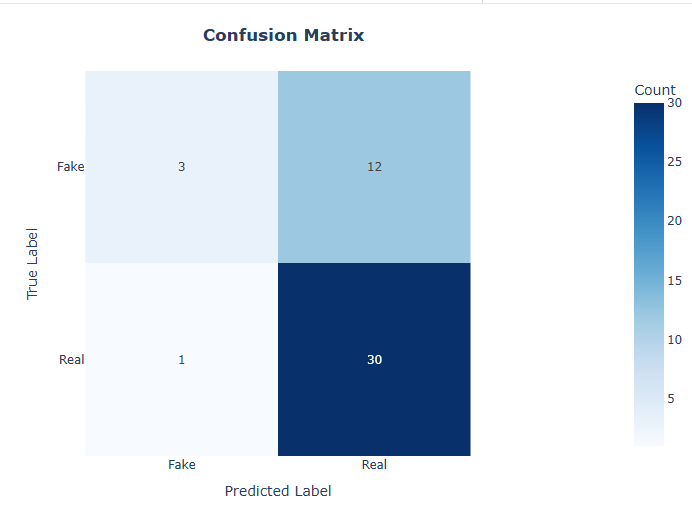
\includegraphics[width=0.78\textwidth]{figures/Confusion_matrix_1.png}
    \caption{Confusion matrix on validation predictions.}
\end{figure}

\begin{figure}[H]
    \centering
    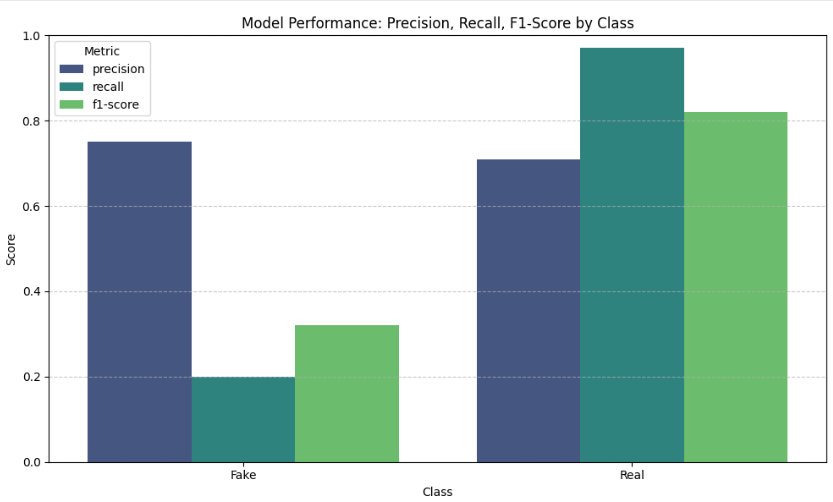
\includegraphics[width=0.78\textwidth]{figures/Precision_recall_F1-score_1.png}
    \caption{Precision, recall, and F1-score by class.}
\end{figure}

\subsection{Error Analysis}
The model predicts almost all samples as \textit{Real}. This yields high recall for real certificates but fails to detect fake certificates. Likely causes include class imbalance, limited forged-pattern diversity, and insufficient discriminative depth in the current architecture. Misclassified fake examples indicate that text-edit artifacts are not consistently captured.

\section{Limitations}
\begin{itemize}[leftmargin=*]
    \item While the current CNN model effectively identifies basic digital forgeries, it has certain limitations due to the experimental environment.
    \item The model's performance is highly dependent on a relatively small dataset of 200 images, which may limit its ability to generalize across highly diverse or unique certificate designs from different countries.
    \item The system currently focuses on visual and textural anomalies but cannot verify the legal validity of the information through a live database or blockchain.
    \item High-resolution forgeries that perfectly replicate original paper textures and fonts may still pose a challenge without additional metadata analysis or multi-modal verification.
\end{itemize}

\section{Future Implementation}
\begin{itemize}[leftmargin=*]
    \item Integrate Optical Character Recognition (OCR) to extract certificate details and cross-verify them with official institutional databases for a two-tier security check.
    \item Deploy the model as a user-friendly web or mobile application so recruiters and institutions can verify documents instantly through smartphone cameras.
    \item Add metadata analysis to detect whether an image file has been processed through editing software.
    \item Train with larger multi-national datasets to improve global accuracy and robustness against sophisticated forgery techniques.
\end{itemize}

% ------------------------
% 7. Conclusion
% ------------------------
\section{Conclusion}
This work demonstrates an end-to-end CNN-based approach for automated competition certificate authenticity detection. The system can capture important visual and textural cues related to forgery and offers a fast, low-cost support tool for verification workflows. Although the current performance indicates class-bias toward real certificates, the proposed enhancements in data diversity, OCR integration, and deployment strategy provide a clear path toward a robust real-world solution.

% ------------------------
% 8. References
% ------------------------
\newpage
\bibliographystyle{IEEEtran}
\bibliography{references}

\end{document}
